\documentclass[../Cours.tex]{subfiles}
\begin{document}

\chapitre{Calcul littéral}


\partie{Expression littérale}

\souspartie{Écriture}
\definition{Une \emph{expression littérale} est un ensemble d'opérations contenant des nombres et des lettres.}
\definition{Dans une expression littérale, une lettre représente un nombre, cette lettre est appelée une \emph{variable}.}

\exemple{$3\times a + 2 \times b$ est une expression littérale contenant 2 variables : $a$ et $b$. Elle est composée de 3 opérations : 2 multiplications et 1 addition.}

\definition{Évaluer une expression signifie remplacer chacune des variables par une valeur numérique donnée.}

\exemple{Évaluer l'expression $3 \times a + 8$ en $a = 2$ signifie remplacer $a$ par 2, ce qui donne :  $3 \times 2 + 8 = 14$.}

\convention{%
Le symbole de multiplication est facultatif entre :
\begin{itemize}
    \item deux variables : $a\times b = ab$
    \item un nombre et une variable : $5 \times x = 5x$
    \item avec une parenthèses : $2 \times (x+3) = 2(x+3)$
\end{itemize}
}

\notation{\vspace{-1.5em}\begin{itemize}
        \item $a \times a = a^2$ (se lit << $a$ au carré >>)
        \item $a \times a \times a = a^2 \times a = a^3$ (se lit << $a$ au cube >>)
    \end{itemize}
}

\begin{listedexemples}
    \item $5^2 = 5 \times 5 = 25$
    \item $2^3 = 2 \times 2 \times 2 = 8$
    \item $h^3 = h \times h \times h$
    \item $(a+b)^2 = (a+b)(a+b)$
\end{listedexemples}

\souspartie{Réduction}

\definition{Réduire une expression, c'est regrouper les termes de même nature/classe/famille.}

\exemple{$2x+3x = 5x$}

\partie{Développement et factorisation}

\souspartie{Somme et produit}

\definition{Une expression littérale est une \emph{somme} lorsque la dernière opération est une addition ou une soustraction.}

\begin{listedexemples}
    \item $3a+b$
    \item $7(2+x)+y$
\end{listedexemples}

\definition{De même, si la dernière opération est une multiplication, on dit que c'est un \emph{produit}.}

\exemple{$3x$ $7(x+y)$ $(a+b)(2a+3b)$}

\souspartie{Distributivité simple}

\definition{Développer, c'est transformer un produit en une somme.}
\definition{Factoriser, c'est transformer une somme en un produit}

\propriete{\textsc{DISTRIBUTIVITÉ}\\ 
\begin{center}
    \begin{tikzpicture}
        \node[anchor=west] at (0,0) {$k(a+b) = ka + kb$};
        \node[anchor=west] at (0,-1.5) {$ka + kb = k(a+b)$};
        \draw[vert,-latex] (0.25,0.3) arc (175:5:0.25);
        \draw[vert,-latex] (0.25,0.3) arc (175:5:0.65 and 0.45);
        \draw[vert] (0.27,-1.5) circle (0.2 and 0.4);
        \draw[vert] (1.45,-1.5) circle (0.2 and 0.4);
    \end{tikzpicture}
\end{center}
}

\clearpage
\EXERCICES
\begin{questions}
    \exercicetitre{Calculs avec priorités}
        Faire chaque calcul, en précisant la nature de la dernière opération effectuée.
        \question $7 + 3 \times 4$
        \question $(7+2) \times (8+3)$
        \question $7 + 8 \times 9 + 3$
        \question $3 + 4 \times 8 \div 2$
        \question $3 \times \left[ 67 - \left( 20 + 45 \right) \right]$
        
    \exercicetitre{Évaluer les expressions}\vspace{-2em}
    \begin{multicols}{2}
        \question Évaluer $2a+5$ en $a=3$
        \question Évaluer $3(b+1)$ en $b=6$
        \question Évaluer $c^2 + 2c$ en $c=4$
        \question Évaluer $4d+d^3$ en $d=5$
    \end{multicols}

    \exercicetitre{Somme ou produit ?}\vspace{-2em}
    \begin{multicols}{3}
        \question $8x+5$
        \question $3x(7x-5)$
        \question $(4\alpha - 2)^2$
        \question $9x^2+5x+1$
        \question $7(x+3) + 6x$
        \question $(4x+2)(6x+1)$
    \end{multicols}

    \exercicetitre{Suite de figures}\vspace{-2em}
    \begin{center}
    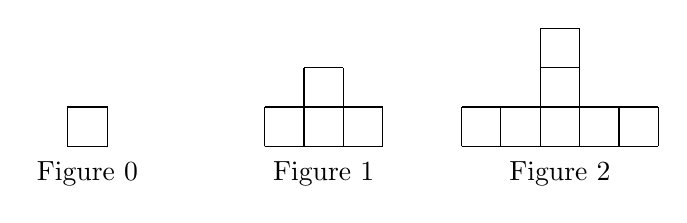
\begin{tikzpicture}[scale=0.5]
        \draw (0,0) rectangle (1,1);
        \node at (0.5,-0.7) {Figure 0};
        \draw (5,0) grid (8,1);
        \draw (6,0) grid (7,2);
        \node at (6.5,-0.7) {Figure 1};
        \draw (10,0) grid (15,1);
        \draw (12,0) grid (13,3);
        \node at (12.5,-0.7) {Figure 2};
    \end{tikzpicture}
    \end{center}

    En poursuivant cette suite de figures, combien y aura-t-il de carrés...
    \question pour la figure 3 ?
    \question pour la figure 10 ?
    \question pour la figure 100 ?
    \question pour la figure $n$ ?

    \exercicetitre{Développer}\vspace{-2em}
    \begin{multicols}{3}
        \question $2(x+8)$
        \question $3(x+2)$
        \question $4x(6+x)$
        \question $3x^2(x+1)$
        \question $25(a+b)$
        \question $y(x+3z)$
    \end{multicols} 

    \exercicetitre{Factoriser}\vspace{-2em}
    \begin{multicols}{3}
        \question $2a + 2b$
        \question $f + 4f^2$
        \question $x^3 + 3x^2$
        \question $9\alpha^2 + 6\alpha + 12$
        \question $35 + 5x$
        \question $9x^2 - 27$
    \end{multicols} 

    \exercicetitre{Sans calculatrice}\vspace{-2em}
    \begin{multicols}{3}
        \question $37 \times 99$
        \question $83 \times 37 + 83 \times 63$
        \question $136 \times 52 - 36 \times 52$
        \question $1001 \times 76$
        \question $0,32 \times 1278 - 0,32 \times 278$
        \question $5,2 \times 3456 + 5,2 \times 6544$
    \end{multicols}
\end{questions}

\clearpage
\CORRECTIONS 

\begin{questions}
    \exercicetitre{Calculs avec priorités}
        \question 
        \begin{align*}
            &7 + \underline{3 \times 4}\\
            &= \underline{7 + 12} \\
            &= \fbox{19}
        \end{align*}
        \question 
        \begin{align*}
            &\underline{(7+2)} \times (8+3) \\
            &= 9 \times \underline{(8+3)} \\
            &= \underline{9 \times 11} \\
            &= \fbox{99}
        \end{align*}
        \question 
        \begin{align*}
            &7 + \underline{8 \times 9} + 3 \\
            &= \underline{7 + 72} + 3 \\
            &= \underline{79 + 3} \\
            &= \fbox{82}
        \end{align*}
        \question 
        \begin{align*}
            &3 + \underline{4 \times 8} \div 2 \\
            &= 3 + \underline{32 \div 2} \\
            &= \underline{3 + 16} \\
            &= \fbox{19}
        \end{align*}
        \question 
        \begin{align*}
            &3 \times \left[ 67 - \left( \underline{20 + 45} \right) \right] \\
            &= 3 \times \left[ \underline{67 - 65} \right] \\ 
            &= \underline{3 \times 2} \\
            &= \fbox{6}
        \end{align*}

    \exercicetitre{Évaluer les expressions}
        \question 
            \begin{align*}
                &2a+5 \\
                &= \underline{2 \times 3} + 5 \\
                &= \underline{6+5} \\
                &= \fbox{11}
            \end{align*}
        \question
            \begin{align*}
                &3(b+1) \\
                &= 3(\underline{6+1}) \\
                &= \underline{3 \times 7} \\
                &= \fbox{21}
            \end{align*}
        \question 
            \begin{align*}
                &c^2+2c \\
                &= 4^2 + 2 \times 4 \\
                &= \underline{4 \times 4} + 2 \times 4 \\
                &= 16 + \underline{2 \times 4} \\
                &= \underline{16 + 8} \\
                &= \fbox{24}
            \end{align*}
        \question 
            \begin{align*}
                &4d + d^3 \\
                &= 4 \times 5 + 5^3 \\
                &= \underline{4 \times 5} + 5 \times 5 \times 5 \\
                &= 20 + \underline{5 \times 5} \times 5 \\
                &= 20 + \underline{25 \times 5} \\
                &= \underline{20 + 125} \\
                &= \fbox{145}
            \end{align*}
\end{questions}

\end{document}